\documentclass[11pt,letterpaper]{article}
\PassOptionsToPackage{hyphens}{url}
\usepackage[margin=.83in,top=.8in,bottom=.8in,headheight=15pt]{geometry}
\usepackage[T1]{fontenc}
\usepackage{lmodern,amsmath,amssymb,mathtools,bm,booktabs,array,graphicx,tikz}
\usetikzlibrary{arrows.meta,positioning,calc,decorations.pathreplacing,patterns}
\definecolor{ink}{HTML}{17344D}\definecolor{accent}{HTML}{087E8B}\definecolor{pale}{HTML}{EDF5F5}\definecolor{gold}{HTML}{AD6B19}
\providecommand{\dd}{\,\mathrm{d}}\providecommand{\R}{\mathbb{R}}
\providecommand{\E}{\mathbb{E}}\providecommand{\Var}{\operatorname{Var}}
\providecommand{\Cov}{\operatorname{Cov}}\providecommand{\diag}{\operatorname{diag}}
\providecommand{\norm}[1]{\left\lVert#1\right\rVert}
\providecommand{\abs}[1]{\left|#1\right|}
\usepackage{microtype,hyperref,fancyhdr,enumitem,amsthm,sectsty,needspace}
\allsectionsfont{\raggedright}
\hypersetup{colorlinks=true,linkcolor=ink,urlcolor=accent,pdfauthor={Zan Ahmad},pdftitle={Functions, control flow, and threshold statistics / Lecture notes}}
\setlength{\parindent}{0pt}\setlength{\parskip}{6pt}\linespread{1.07}
\setlist{itemsep=3pt,topsep=4pt,leftmargin=*}
\emergencystretch=2em\clubpenalty=10000\widowpenalty=10000
\pagestyle{fancy}\fancyhf{}\fancyhead[L]{\small Scientific Computing in Python}\fancyhead[R]{\small Lecture 2}
\fancyfoot[L]{\footnotesize Zan Ahmad}\fancyfoot[R]{\footnotesize\thepage}\renewcommand{\headrulewidth}{.3pt}
\newtheorem{proposition}{Proposition}\newtheorem{theorem}{Theorem}\newtheorem{lemma}{Lemma}
\theoremstyle{definition}\newtheorem{definition}{Definition}\newtheorem{example}{Example}
\numberwithin{equation}{section}
\begin{document}
{\small\scshape Scientific Computing in Python\hfill Lecture 2}\par\medskip
{\raggedright\hyphenpenalty=10000\exhyphenpenalty=10000\LARGE\bfseries\color{ink} Functions, control flow, and threshold statistics\par}\medskip
{\small Lecture notes}\par\bigskip
A threshold calculation is a useful setting for functions and loops because its mathematical definition is short and its exceptional cases are visible. We shall distinguish a known measurement from a missing value, count the observations satisfying a stated inequality, and identify the first recorded qualifying time. The inequality and the denominator are parts of the statistic.

\section{A three-valued classification rule}
\hypertarget{note-a-three-valued-classification-rule}{}\label{note:a-three-valued-classification-rule}
{\small \href{slides.html\#frame=a-three-valued-classification-rule\&step=1}{Slides for this section}}\par
Let $x$ be a reading and let $\theta$ be a fixed threshold. A missing reading has no numerical order relative to $\theta$ and must be handled before comparison. For a known reading the two cases $x\leq\theta$ and $x>\theta$ are disjoint and exhaustive. Equality belongs to the first case. The function implements precisely this partition.

\[
c(x;\theta)=\begin{cases}\text{missing},&x\text{ absent},\\\text{at or below},&x\leq\theta,\\\text{above},&x>\theta.\end{cases}
\]

At $\theta=40$, the values $40$ and $40.1$ belong to different classes.

\subsection*{A function implementing the partition}
\begin{minipage}{\linewidth}
\begin{verbatim}
def classify(value, target):
    if value is None:
        return "missing"
    if value <= target:
        return "at_or_below"
    return "above"
\end{verbatim}
\end{minipage}
\section{Arguments, returns, and local names}
\hypertarget{note-arguments-returns-and-local-names}{}\label{note:arguments-returns-and-local-names}
{\small \href{slides.html\#frame=arguments-returns-and-local-names\&step=1}{Slides for this section}}\par
A function receives values through its parameters and produces a value with return. A return statement ends that invocation immediately. Local variables belong to the current call. Printing a result displays text but does not replace returning a result for use in another calculation. A function that depends only on explicit arguments is easier to reason about than one whose threshold is stored in a mutable global variable.

\begin{minipage}{\linewidth}
\begin{verbatim}
category = classify(35, 40)
print(category)
\end{verbatim}
\end{minipage}

The returned string is a value. The function can be called again with a different threshold without changing its definition.

\subsection*{Boundary cases}
\begin{center}\begin{tabular}{lll}\toprule
Reading & Threshold & Category\\\midrule
\texttt{None}&40&missing\\40&40&at or below\\40.1&40&above\\\bottomrule\end{tabular}\end{center}

Testing the boundary establishes whether the implemented inequality agrees with the definition.
\section{Indicators and accumulated counts}
\hypertarget{note-indicators-and-accumulated-counts}{}\label{note:indicators-and-accumulated-counts}
{\small \href{slides.html\#frame=indicators-and-accumulated-counts\&step=1}{Slides for this section}}\par
For known readings define $I_i(\theta)=1$ when $x_i\leq\theta$ and zero otherwise. The qualifying count is the sum of these indicators. A loop calculates that sum one contribution at a time. After processing the first $k$ observations, the three counters must sum to $k$. This is a loop invariant: initialization makes it true, and each iteration preserves it by incrementing exactly one counter.

\[
N_{\leq}(\theta)=\sum_{i:\,x_i\text{ known}}\mathbf1_{\{x_i\leq\theta\}}.
\]

After $k$ observations,
\[
N_{\leq}^{(k)}+N_{>}^{(k)}+N_{\rm missing}^{(k)}=k.
\]

\subsection*{The nine-reading example}
\[
80,62,48,40,35,\text{missing},28,25,23.
\]
At threshold $40$:

\[
N_{\leq}=5,\quad N_>=3,\quad N_{\rm missing}=1.
\]
The counter identity gives $5+3+1=9$.
\begin{center}\begin{minipage}{.98\linewidth}\centering
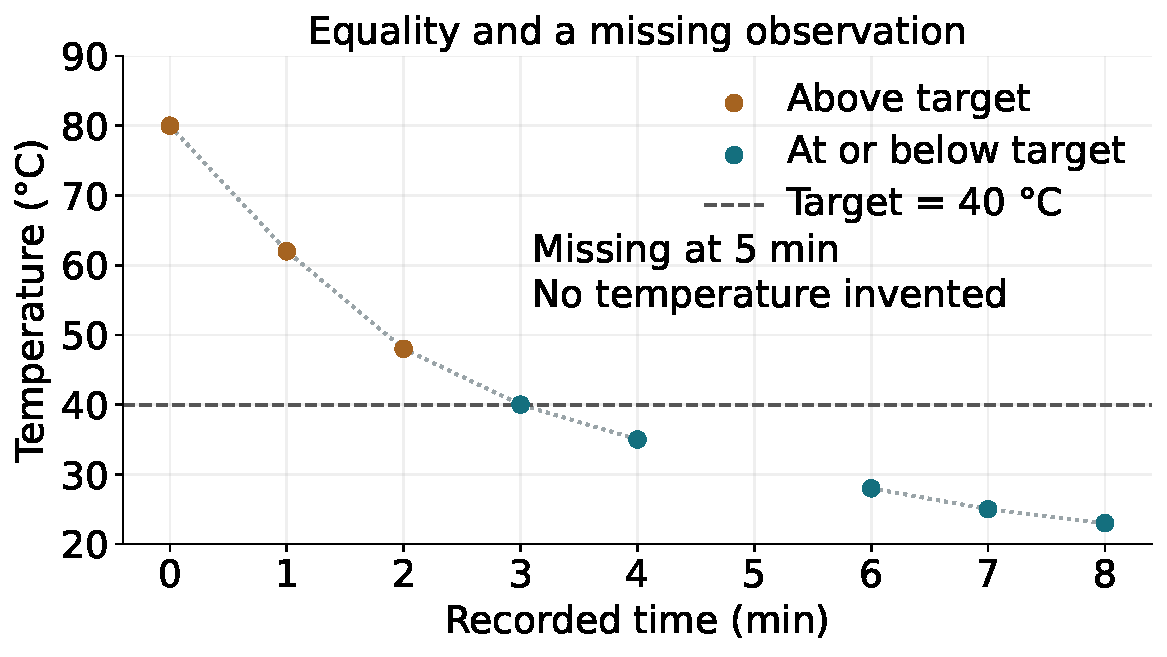
\includegraphics[width=.96\linewidth,height=.57\textheight,keepaspectratio]{presentation-figures/threshold-record.pdf}\par\smallskip
{\small The equality case at minute 3 qualifies; the missing reading at minute 5 is left absent. Dotted connectors are visual aids only.}
\end{minipage}\end{center}
\section{The denominator of a proportion}
\hypertarget{note-the-denominator-of-a-proportion}{}\label{note:the-denominator-of-a-proportion}
{\small \href{slides.html\#frame=the-denominator-of-a-proportion\&step=1}{Slides for this section}}\par
A proportion must identify its reference group. Among known readings the qualifying fraction is $N_{\leq}/N_{\rm known}$, where $N_{\rm known}=N_{\leq}+N_>$. Counting a missing reading as a failure silently changes the reference group. If every value is missing the denominator is zero and the proportion is undefined. The function should represent that case explicitly.

\[
f(\theta)=\frac{N_{\leq}(\theta)}{N_{\rm known}},\qquad N_{\rm known}>0.
\]

For the supplied record,
\[
f(40)=\frac58=0.625.
\]

\subsection*{Changing the threshold}
At threshold $35$, only $35,28,25,23$ qualify:
\[
f(35)=\frac48=0.5.
\]

The known-reading denominator remains $8$ because the data and missingness did not change.
\section{The first recorded qualifying time}
\hypertarget{note-the-first-recorded-qualifying-time}{}\label{note:the-first-recorded-qualifying-time}
{\small \href{slides.html\#frame=recorded-threshold-attainment-figure\&step=1}{Slides for this section}}\par
The first recorded qualifying time is the minimum of a subset of observation times. An empty subset has no minimum, so we use None to represent the absence of a qualifying reading. Time zero is a valid result and must not be confused with absence. Once the first time has been assigned, subsequent qualifying observations must leave it unchanged.

\[
t_{\rm first}=\min\{t_i:x_i\text{ known and }x_i\leq\theta\}.
\]

For observations at integer minutes and $\theta=40$, $t_{\rm first}=3$ min.

\subsection*{Recorded time and continuous crossing}
The record contains $T(2)=48$ and $T(3)=40$.

The first qualifying observation occurs at $3$ min. An exact continuous crossing requires a model between observations. With oscillation, even earlier unobserved crossings are possible.
\begin{center}\begin{minipage}{.98\linewidth}\centering
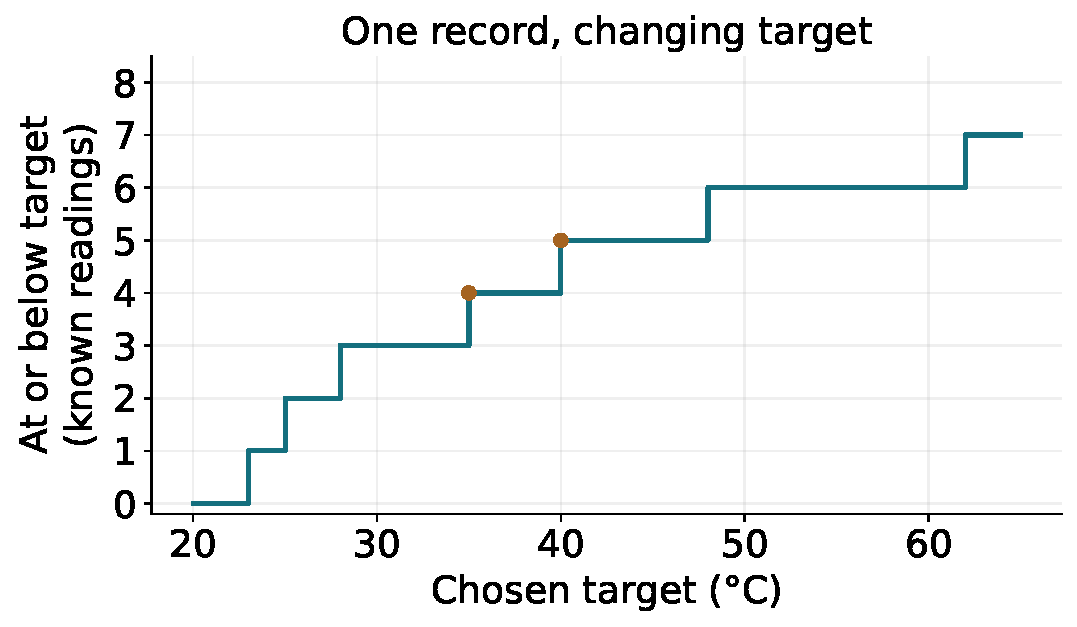
\includegraphics[width=.96\linewidth,height=.57\textheight,keepaspectratio]{presentation-figures/threshold-counts.pdf}\par\smallskip
{\small The at-or-below count is nondecreasing as the target increases; data and missingness remain fixed.}
\end{minipage}\end{center}
\section{Monotonicity of threshold counts}
\hypertarget{note-monotonicity-of-threshold-counts}{}\label{note:monotonicity-of-threshold-counts}
{\small \href{slides.html\#frame=changing-the-threshold\&step=1}{Slides for this section}}\par
If $\theta_1\leq\theta_2$, every observation qualifying at $\theta_1$ also qualifies at $\theta_2$. Thus the qualifying count is nondecreasing in the threshold. For fixed data it is a step function, with jumps at observed values. This mathematical property provides a test across many thresholds without specifying every answer separately.

\[
\{i:x_i\leq\theta_1\}\subseteq\{i:x_i\leq\theta_2\}
\quad(\theta_1\leq\theta_2).
\]

Therefore $N_{\leq}(\theta_1)\leq N_{\leq}(\theta_2)$.

\subsection*{A loop with paired observations}
\begin{minipage}{\linewidth}
\begin{verbatim}
for time, value in zip(times, readings):
    category = classify(value, target)
    counts[category] += 1
    if category == "at_or_below" and first is None:
        first = time
\end{verbatim}
\end{minipage}
Equal list lengths must be checked: \texttt{zip} stops at the shorter input.
\bigskip
\section*{Exercises}
\par\noindent\begin{minipage}{\linewidth}
\subsection*{H2-1. Trace the decision boundary}
Use target 37 degrees Celsius and readings [None, 37, 37.1, 36.9]. New practice; 10 feedback points.

\textbf{a} Give the category of each reading in order for an at-or-below rule.

\end{minipage}\par\medskip
\textbf{b} State the known-reading denominator and qualifying fraction.

\textbf{c} How do the count and fraction change if the rule is strictly below?

\par\noindent\begin{minipage}{\linewidth}
\subsection*{H2-2. Keep the first qualifying time}
Times are [0, 2, 4, 6] minutes and temperatures are [35, 44, None, 34] degrees Celsius. Target: 35 degrees. New practice; 10 feedback points.

\textbf{a} Trace the qualifying count and stored first time after each observation.

\end{minipage}\par\medskip
\textbf{b} Explain the bug in replacing a test of first\_time is None with not first\_time.

\textbf{c} What can this record establish about an exact continuous crossing time?

\par\noindent\begin{minipage}{\linewidth}
\subsection*{H2-3. Write and check a reusable rule}
Work with small supplied numeric inputs and None. New practice; 10 feedback points.

\textbf{a} Give the complete ordered decision logic for a function with a reading and a target as inputs. It must return one of missing, at\_or\_below or above.

\end{minipage}\par\medskip
\textbf{b} Give three test calls that distinguish boundary, above-boundary and missing behavior, with expected results.

\textbf{c} Explain why printing the label without returning it is insufficient for a later counting function.

\par\noindent\begin{minipage}{\linewidth}
\subsection*{H2-4. Interpret missingness and a changing target}
A new record contains [12, None, 18, 21, None] degrees Celsius. New practice; 10 feedback points.

\textbf{a} For target 18 degrees, give all category counts and the fraction among known readings.

\end{minipage}\par\medskip
\textbf{b} Prove in words that raising the target cannot decrease the qualifying count when data are fixed.

\textbf{c} If every reading were None, what should a report say about the qualifying fraction, and why?

\section*{References}
\noindent\begin{minipage}{\linewidth}
Original Python Lecture 0. PDF pages 44--45 and 47--49.

\url{https://zanahmad.com/files/scientific-python/Lecture_0__Intro_to_Python.pdf}
\end{minipage}\par\medskip
\noindent\begin{minipage}{\linewidth}
Original Python Lecture 1. PDF pages 4--9.

\url{https://zanahmad.com/files/scientific-python/Lecture_1__Intro_to_Python.pdf}
\end{minipage}\par\medskip
Python source materials: Phillip Kerger (2023). Course adaptation and additional exposition: Zan Ahmad.

\end{document}
